\documentclass[12pt,a4paper]{article}

\usepackage{booktabs}
\usepackage{longtable}
\usepackage{pdflscape}
\usepackage{graphicx}
\usepackage{float}
\usepackage{caption}
\usepackage{amsmath}
\usepackage{threeparttable}
\usepackage{geometry}
\usepackage[table]{xcolor}
\usepackage{chngcntr}
\geometry{margin=2.5cm}

\title{ISOs Diffusion in the EU: an Endogenous Network Recovery for
       Environmental and Quality Management Systems}
\author{Gianluigi De Rubertis}
\date{\today}

\begin{document}

\maketitle

\begin{abstract}
    Your abstract text here.
\end{abstract}

\newpage

\tableofcontents

\newpage

\section {Introduction}
The study identifies political and techincal standards, represented by ISO 14001 (Environmental Management) and ISO 9001 (Quality Management) respectively, as paradigmatic cases of policy diffusion in the EU. It applies the De Paula, Rasul \& Souza (2025) method to recover peer effects and networks of influence from panel data on ISO certifications across 27 EU countries over 1993--2017. The recovered networks are compared to exogenous benchmarks based on geography, trade, culture and institutional similarity, and used to estimate peer effects via IV-2SLS with country FE. The paper contributes to the literature on peer effects and network formation (Manski 1993; Bramoullé et al., 2009; De Paula, Rasul \& Souza 2025), policy diffusion (Berliner \& Prakash 2013) and ISO standards diffusion (Guler et al., 2002; Albuquerque et al., 2007).

\subsection{Literature Review}

\begin{itemize}
    \item \textbf{Peer effects and network formation:} Manski (1993) establishes the reflection problem in identifying social effects; Bramoullé et al. (2009) show identification via network exclusion restrictions; De Paula, Rasul \& Souza (2025) extend this to unknown networks via penalised GMM.
    \item \textbf{Policy diffusion:} Berliner \& Prakash (2013) document the role of weak governance in driving voluntary standard adoption as a signalling device.
    \item \textbf{ISO standards diffusion:} Guler et al. (2002) identify trade and foreign investment as channels of ISO 9001 diffusion; Albuquerque et al. (2007) provide spatiotemporal evidence of cross-country spillovers for both ISO 9001 and ISO 14001.
\end{itemize}

\section {Data and Methodology}
\subsection{Data} \textit{Data.} Country-level annual counts of valid ISO 9001 and ISO 14001 certificates from the ISO Survey, covering 27 EU countries over 1993--2017 for Quality and 1997--2017 for Environment ($N=27$, $T=25$ and $T=21$ respectively). Covariates from the World Bank WDI: GDP per capita, Trade (\% of GDP), Renewables (\%), Natural Resources Rents (\% of GDP); Rule of Law from the Worldwide Governance Indicators (WGI).
\subsection{Methodology} De Paula, Rasul \& Souza (2025) extend the peer-effects literature (Manski 1993; Bramoullé et al., 2009) to the case in which the network of interactions is unknown. Their structural model \begin{equation} y_{it} = \rho_0 \sum_{j=1}^{N} W_{0,ij}\, y_{jt} + \beta_0 x_{it} + \gamma_0 \sum_{j=1}^{N} W_{0,ij}\, x_{jt} + \alpha_i + \alpha_t + \varepsilon_{it} \label{eq:structural} \end{equation} admits the compact form $y_t = \rho_0 W_0 y_t + \beta_0 x_t + \gamma_0 W_0 x_t + \varepsilon_t$, which rearranges into the reduced form \begin{equation} y_t = \Pi_0 x_t + \nu_t, \qquad \Pi_0 = (I - \rho_0 W_0)^{-1}(\beta_0 I + \gamma_0 W_0). \label{eq:reduced} \end{equation} If $W_0$ were known, equation~\eqref{eq:reduced} would directly identify the structural parameters $(\rho_0,\beta_0,\gamma_0)$ from a reduced-form regression of outcomes on covariates (Bramoullé et al., 2009). The contribution of De Paula, Rasul \& Souza is to show that, when $W_0$ is unknown, $\Pi_0$ still contains enough information to recover both the network and the parameters jointly. The intuition is the one that underlies any diffusion process. If a contagious disease spreads through a population, the people who fall ill at the same time tend to be the ones who interact: knowing who got sick when, and what their characteristics are, one can work backwards to who must have been in contact with whom. The same logic applies here. If four countries adopt a standard in synchronous patterns that cannot be explained by their own characteristics alone, the synchrony itself is evidence of a link between them. Cross-country covariation in $y$, conditional on $x$, identifies who is connected to whom, and the strength of the covariation, suitably disentangled, identifies how strong the link is. In principle, $\Pi_0$ is identified as the linear projection of $y$ on $x$ and could be recovered by ordinary least squares whenever the panel is long enough relative to the number of parameters. In typical short panels this is infeasible. De Paula, Rasul \& Souza recover the network $\hat W$ jointly with the structural parameters $(\hat\rho, \hat\beta, \hat\gamma)$ via an adaptive elastic-net GMM (Caner \& Zhang 2014) defined directly on the moment conditions implied by the structural model. Sparsity in $\hat W$ regularises the high-dimensional problem and restores consistency in short panels, estimating the network from observed spillovers without requiring a priori commitment to any specific weighting scheme.
% =============================================================================
\section{EU: Quality (ISO 9001) versus Environment (ISO 14001)}
% =============================================================================

\subsection{Descriptive Statistics}

\begin{table}[H]\centering
\caption{Descriptive statistics}
\label{tab:desc_stats}
\begin{tabular}{lcccccc}\hline\hline
& \multicolumn{3}{c}{Quality (ISO 9001)} & \multicolumn{3}{c}{Environment (ISO 14001)} \\
\cmidrule(lr){2-4} \cmidrule(lr){5-7}
& 1993 & 1999 & 2017 & 1993 & 1999 & 2017 \\\hline
Countries Number & 27 & 27 & 27 & & 27 & 27 \\
Total & 8,866 & 115,052 & 315,987 & & 4,996 & 84,316 \\
Mean & 328.4 & 4,261.2 & 11,703.2 & & 185.0 & 3,122.8 \\
Std.\ Dev. & 508.9 & 7,289.6 & 21,695.1 & & 268.9 & 4,020.2 \\
Min--Max & 0--1,586 & 39--30,150 & 191--97,646 & & 0--962 & 35--14,571 \\
Cert./GDP p.c. & 11.52 & 158.51 & 441.67 & & 6.44 & 128.86 \\
\hline\hline
\multicolumn{7}{p{0.92\textwidth}}{\footnotesize \textit{Notes:} This table summarises the distribution of certifications across the 27 EU countries in the three selected years. The first row reports the number of countries with non-missing data in each year, which is the basis for all subsequent statistics. The second row reports the total number of certifications across all countries, while the third and fourth rows report the mean and standard deviation of certifications per country, respectively. The fifth row reports the minimum and maximum number of certifications across countries. Finally, the sixth row reports the mean certification intensity, defined as the number of certifications per thousand dollars of GDP per capita, averaged across countries. Environment 1993 is empty as its adoption started in 1997. Sources: ISO Survey, World Bank.} \\
\end{tabular}
\end{table}


% =============================================================================
\subsection{Network Recovery}
% =============================================================================

% --- methodology prose here ---

\begin{table}[H]\centering
\caption{BIC-selected networks}\label{tab:network_eu}
\begin{tabular}{lcc}\hline\hline
& Quality & Environment \\\hline
Number of links & 28 & 30 \\
Links in both networks & 3 & 3 \\
Clustering & 0.164 & 0.053 \\
Reciprocated links & 7.1\% & 0.0\% \\
Degree distribution across nodes (countries) & & \\
\quad Out-degree & 1.037 (0.338) & 1.111 (0.698) \\
\quad In-degree & 1.037 (1.372) & 1.111 (1.219) \\
\hline
$\hat{\rho}$ (GMM) & 0.2025 & 0.2864 \\
$\lambda$ & (0.100, 0.150, 0.200) & (0.050, 0.050, 0.100) \\
BIC & 13.96 & 14.57 \\
\hline\hline
\multicolumn{3}{p{0.95\textwidth}}{\footnotesize \textit{Notes:} This table reports summary statistics of the two recovered networks, selected by BIC. The first row reports the number of links in each network, while the second and third rows report how many links are shared by both networks and how many are unique to each network, respectively. A shared link is intended when there is a link between the same two nodes in the same direction in both networks. The fourth and fifth rows report the clustering coefficient (share of closed triplets) and reciprocity (bidirectional links) of each network, respectively. The sixth to ninth rows report the mean and standard deviation of out-degrees and in-degrees across nodes (countries) for each network. Finally, the tenth to twelfth rows report the GMM estimates of the structural parameter $\hat{\rho}$ (endogenous peer effects) and tuning paramters $\hat{\lambda}$ and the BIC values for each network.} \\
\end{tabular}\end{table}


% =============================================================================
\subsection{Recovered Networks}
% =============================================================================

\begin{figure}[H]
    \centering
    \caption{Recovered networks}
    \label{fig:networks}
    \includegraphics[width=\textwidth]{assets/figures/networks_weighted_full}
    \par\vspace{0.5em}
    {\footnotesize \textit{Notes.} Quality and Environment networks recovered via De Paula, Rasul \& Souza (2025). Networks are weighted and directed. Each is shown in its own Fruchterman--Reingold layout (Quality--Quality and Environment--Environment) and in the other standard's layout (Quality--Environment and Environment--Quality) to facilitate visual comparison of topology.}
\end{figure}


% =============================================================================
\subsection{Peer Effects: Recovered vs Exogenous Networks}
% =============================================================================

\begin{figure}[H]
    \centering
    \caption{Peer-effect estimates across network specifications.}
    \label{fig:bdf_combined}
    \includegraphics[width=\textwidth]{assets/figures/bdf_forest_combined}
    \par\vspace{0.5em}
    {\footnotesize \textit{Notes.} \textit{Observations:} Quality $N \times T = 624$ (simultaneous), $598$ (lagged); Environment $N \times T = 468$ (simultaneous), $442$ (lagged). The figure reports IV-2SLS peer-effect estimates ($\hat\beta$) and 95\% confidence intervals from the Bramoullé, Djebbari \& Fortin (2009) linear-in-means specification, estimated on the recovered networks (De Paula, Rasul \& Souza 2025) and on the exogenous benchmark networks of Albuquerque et al.\ (2007). Error bars are cluster-bootstrapped (999 draws, country clusters). Within-$R^2$ labelled above each point estimate. The two panels show results with and without a one year lag. Slovenia dropped (isolated node in the recovered Quality network).}
\end{figure}

\begin{figure}[H]
    \centering
    \caption{Simulation Results, Adaptive Elastic-Net GMM}
    \label{fig:depaula_appendix}
    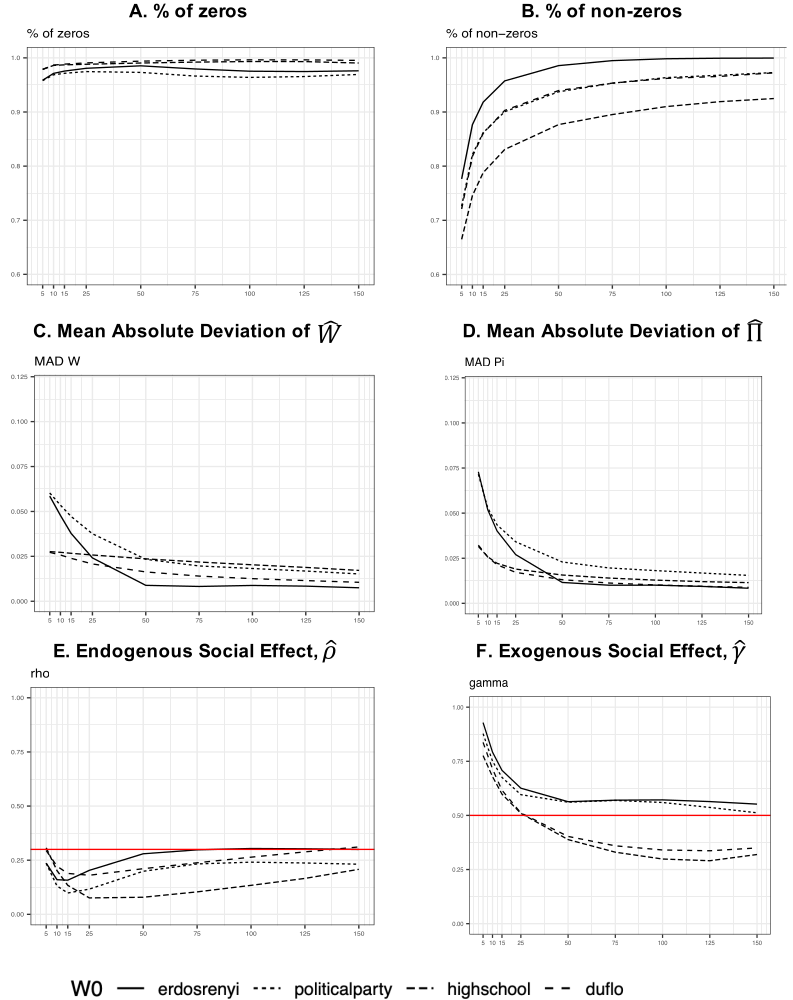
\includegraphics[width=\textwidth]{assets/figures/depaula_appendix_figure.png}
    \par\vspace{0.5em}
    {\footnotesize \textit{Notes.} \textit{Source:} De Paula, Rasul \& Souza (2025), Figure A1. Results from 1000 Monte Carlo iterations under various true networks and time periods $T = 25, 50, 75, 100, 125, 150$, with true parameters $\rho_0 = 0.3$, $\beta_0 = 0.4$, $\gamma_0 = 0.5$. Panel A: share of true zero elements in $W$ estimated below $0.05$. Panel B: share of true non-zero elements above $0.3$ estimated as non-zero. Panels C--D: mean absolute deviation of the estimated network from the true $W$ and reduced-form matrix respectively. Panels E--F: recovered parameters averaged across iterations; true values marked by horizontal red lines. All specifications include time and node fixed effects.}
\end{figure}

\clearpage

% =============================================================================
\subsection{Network Similarity}
% =============================================================================
To assess how closely the two recovered networks $\hat W^Q$ and $\hat W^E$ overlap, we summarise their structural similarity through the \textbf{Jaccard index} (Jaccard 1901; Wasserman \& Faust 1994, Sec.\ 11.4): \begin{equation} J(\hat W^Q, \hat W^E) = \frac{|E_Q \cap E_E|}{|E_Q \cup E_E|}, \label{eq:jaccard} \end{equation} where $E_Q = \{(i, j) : |\hat w^Q_{ij}| > 10^{-5}\}$ and $E_E$ is defined analogously. The index ranges in $[0, 1]$, with $J = 0$ for disjoint networks and $J = 1$ for identical edge sets. For the BIC-selected recovered networks, $|E_Q| = `r n_q`$, $|E_E| = `r n_e`$, $|E_Q \cap E_E| = `r n_inter`$, and $|E_Q \cup E_E| = `r n_union`$, yielding $J = `r jaccard_val`$.

\input{assets/tables/network_jaccard_summary}

\begin{table}[!h]
\centering
\caption{\label{tab:jaccard_similarity_quality}Jaccard similarity matrix: Quality networks.}
\centering
\fontsize{9}{11}\selectfont
\begin{threeparttable}
\begin{tabular}[t]{llcccc}
\toprule
  & Recovered & Geo + Trade & Geography & Trade & Cultural dist.\\
\midrule
Recovered & 1.000 &  &  &  & \\
Geo + Trade & 0.170 & 1.000 &  &  & \\
Geography & 0.124 & 0.604 & 1.000 &  & \\
Trade & 0.101 & 0.604 & 0.209 & 1.000 & \\
Cultural dist. & 0.111 & 0.181 & 0.157 & 0.141 & 1.000\\
\bottomrule
\end{tabular}
\begin{tablenotes}[para]
\item \textit{Notes:} 
\item This table shows the lower triangle only of the similarity matrix based on the Jaccard index for all the Quality networks considered in this paper. A link is active if $w_{ij} > 0$.
\end{tablenotes}
\end{threeparttable}
\end{table}


\begin{table}[!h]
\centering
\caption{\label{tab:tab:jaccard_similarity_environment}Jaccard similarity matrix: Environment networks.}
\centering
\fontsize{9}{11}\selectfont
\begin{threeparttable}
\begin{tabular}[t]{llcccc}
\toprule
  & Recovered & Geo + Culture & Geography & Trade & Cultural dist.\\
\midrule
Recovered & 1.000 &  &  &  & \\
Geo + Culture & 0.168 & 1.000 &  &  & \\
Geography & 0.097 & 0.579 & 1.000 &  & \\
Trade & 0.114 & 0.214 & 0.209 & 1.000 & \\
Cultural dist. & 0.107 & 0.579 & 0.157 & 0.141 & 1.000\\
\bottomrule
\end{tabular}
\begin{tablenotes}[para]
\item \textit{Notes:} 
\item This table shows the lower triangle only of the similarity matrix based on the Jaccard index for all the Environment networks considered in this paper. A link is active if $w_{ij} > 0$.
\end{tablenotes}
\end{threeparttable}
\end{table}


\clearpage

% =============================================================================
\subsection{Dyadic Regression}
% =============================================================================

% --- prose motivating the dyadic regression here ---


\begin{table}[htbp]
   \caption{\label{tab:dyadic_recovered_fp_lpm} Dyadic determinants of the recovered network: continuous link weight (OLS) and link presence (LPM), with sender and receiver fixed effects, full-period averages (1993--2017).}
   \centering
   \begin{tabular}{lcccc}
      \tabularnewline \midrule \midrule
        & \multicolumn{2}{c}{Quality} & \multicolumn{2}{c}{Environment} \\ 
      Outcome                                 & Weight (OLS)  & Binary (LPM) & Weight (OLS)  & Binary (LPM) \\   
                                              & (1)           & (2)          & (3)           & (4)\\  
      \midrule
      \emph{Variables}\\
      Economic distance                       & -0.0338       & -0.0357      & -0.0360$^{*}$ & -0.0289\\   
                                              & (0.0244)      & (0.0255)     & (0.0207)      & (0.0214)\\   
      Env. policy asymmetry                   & 0.0190        & 0.0081       & 0.0381$^{**}$ & 0.0386$^{*}$\\   
                                              & (0.0215)      & (0.0219)     & (0.0178)      & (0.0206)\\   
      Cultural distance                       & 0.0009        & 0.0011       & 0.0002        & $-5.29\times 10^{-5}$\\    
                                              & (0.0006)      & (0.0007)     & (0.0004)      & (0.0005)\\   
      Geographic distance                     & -0.0173       & -0.0244      & -0.0037       & 0.0029\\   
                                              & (0.0169)      & (0.0202)     & (0.0179)      & (0.0214)\\   
      Bilateral FDI                           & 0.0143$^{**}$ & 0.0130$^{*}$ & 0.0018        & 0.0040\\   
                                              & (0.0064)      & (0.0065)     & (0.0067)      & (0.0077)\\   
      Bilateral Trade (log)                   & 0.0031        & 0.0057       & -0.0031       & -0.0027\\   
                                              & (0.0042)      & (0.0055)     & (0.0049)      & (0.0049)\\   
      \midrule
      \emph{Fixed-effects}\\
      Sender FE ($\alpha_i^{\text{out}}$):    & Yes           & Yes          & Yes           & Yes\\  
      Receiver FE ($\alpha_j^{\text{in}}$):   & Yes           & Yes          & Yes           & Yes\\  
      \midrule
      \emph{Fit statistics}\\
      Observations                            & 702           & 702          & 702           & 702\\  
      R$^2$                                   & 0.08855       & 0.10533      & 0.06667       & 0.07247\\  
      \midrule \midrule & \tabularnewline
   \end{tabular}
   
   \par \raggedright 
   \textit{Notes} The \emph{Weight} columns regress the recovered weight $\hat w_{ij}$ by OLS; the \emph{Presence} columns regress the binary link indicator $\mathbf{1}(\hat w_{ij}>10^{-5})$ by linear probability model. Sample: 702 directed pairs, 27 EU countries, full-period (1993--2017) averages. Two-way clustered SE (sender $\times$ receiver). Significance: $^{***}$ $p<0.01$, $^{**}$ $p<0.05$, $^{*}$ $p<0.10$.
\end{table}





\clearpage

% =============================================================================
\appendix
\section{Appendix}
\renewcommand{\thefigure}{A\arabic{figure}}
\renewcommand{\thetable}{A\arabic{table}}
\setcounter{figure}{0}
\setcounter{table}{0}
% =============================================================================

\subsection{Grid Search Results}

\begin{table}[!h]
\centering
\caption{\label{tab:tab:grid_search}Top-5 BIC grid search results per standard. BIC-selected specification in bold.}
\centering
\fontsize{9}{11}\selectfont
\begin{threeparttable}
\begin{tabular}[t]{lcccrrr}
\toprule
Panel & $\lambda_1$ & $\lambda_2$ & $\lambda_1^*$ & Edges & $\hat\rho_{GMM}$ & BIC\\
\midrule
\cellcolor[HTML]{FFF9C4}{\textbf{Environment}} & \cellcolor[HTML]{FFF9C4}{\textbf{0.050}} & \cellcolor[HTML]{FFF9C4}{\textbf{0.050}} & \cellcolor[HTML]{FFF9C4}{\textbf{0.100}} & \cellcolor[HTML]{FFF9C4}{\textbf{30}} & \cellcolor[HTML]{FFF9C4}{\textbf{0.286}} & \cellcolor[HTML]{FFF9C4}{\textbf{14.57}}\\
Environment & 0.050 & 0.050 & 0.150 & 30 & 0.287 & 14.57\\
Environment & 0.050 & 0.050 & 0.200 & 30 & 0.288 & 14.57\\
Environment & 0.050 & 0.100 & 0.100 & 31 & 0.277 & 14.62\\
Environment & 0.050 & 0.150 & 0.050 & 31 & 0.276 & 14.62\\
\addlinespace
\cellcolor[HTML]{FFF9C4}{\textbf{Quality}} & \cellcolor[HTML]{FFF9C4}{\textbf{0.100}} & \cellcolor[HTML]{FFF9C4}{\textbf{0.150}} & \cellcolor[HTML]{FFF9C4}{\textbf{0.200}} & \cellcolor[HTML]{FFF9C4}{\textbf{28}} & \cellcolor[HTML]{FFF9C4}{\textbf{0.203}} & \cellcolor[HTML]{FFF9C4}{\textbf{13.96}}\\
Quality & 0.150 & 0.100 & 0.150 & 29 & 0.276 & 14.25\\
Quality & 0.150 & 0.100 & 0.200 & 29 & 0.280 & 14.26\\
Quality & 0.150 & 0.150 & 0.200 & 30 & 0.255 & 14.30\\
Quality & 0.100 & 0.150 & 0.150 & 31 & 0.181 & 14.31\\
\bottomrule
\end{tabular}
\begin{tablenotes}[para]
\item \textit{Notes:} 
\item Top 5 penalisation parameter combinations by BIC, from a grid search over the adaptive elastic-net GMM estimator of De Paula, Rasul and Souza (2025). The BIC-selected specification is highlighted in yellow. Convergence failures are denoted by ---.
\end{tablenotes}
\end{threeparttable}
\end{table}



\subsection{Degree Distributions}

\begin{figure}[H]
    \centering
    \caption{Degree distributions of recovered networks}
    \label{fig:degree_hist}
    \includegraphics[width=\textwidth]{assets/figures/degree_hist}
    \par\vspace{0.5em}
    {\footnotesize \textit{Notes.} This figure shows the in- and out-degree distributions of the recovered Quality and Environment networks. Degree is defined as the number of non-zero entries in each row (out-degree) or column (in-degree) of the recovered weight matrix $\hat W$.}
\end{figure}

\subsection{GMM Parameter Estimates}

\begin{figure}[H]
    \centering
    \caption{GMM parameter estimates}
    \label{fig:gmm_ci}
    \includegraphics[width=0.85\textwidth]{assets/figures/gmm_ci}
    \par\vspace{0.5em}
    {\footnotesize \textit{Notes.} This figure shows the point estimates and 95\% confidence intervals for the GMM parameters $(\rho, \beta, \gamma)$ from the network recovery step. Estimates are shown separately for the Quality and Environment standards. Error bars are based on the asymptotic sandwich variance estimator that conditions on the recovered network $\hat W$ (De Paula, Rasul \& Souza 2025).}
\end{figure}

\end{document}